\newpage
\section{84. 柱状图中最大的矩形}
\label{leetcode:84}

\subsection{题目}

给定 n 个非负整数,用来表示柱状图中各个柱子的高度。每个柱子彼此相邻,且宽度为 1 。

求在该柱状图中,能够勾勒出来的矩形的最大面积。

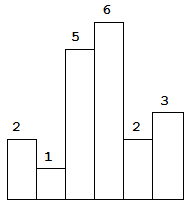
\includegraphics[width=50mm,height=50mm]{images/leetcode/histogram.png}

以上是柱状图的示例,其中每个柱子的宽度为 1,给定的高度为 [2,1,5,6,2,3]。

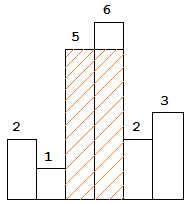
\includegraphics[width=50mm,height=50mm]{images/leetcode/histogram_area.png}

图中阴影部分为所能勾勒出的最大矩形面积,其面积为 10 个单位。

\textbf{示例}:

\begin{verbatim}
  输入: [2,1,5,6,2,3]
  输出: 10
\end{verbatim}

\subsection{参考题解,暴力法}

先用两重循环遍历出所有可能的左右边界组合。
比如我把左边界叫做 left,右边界叫做 right,
然后我们在 left 和 right 之间去找最矮的那根柱子,
那么面积就是 (right - left) * 最矮柱子的高度。

\begin{verbatim}
/**
 * @param {number[]} heights
 * @return {number}
 */
var largestRectangleArea = function(heights) {
  // 暴力解法,会超出时间限制。
  let maxarea = 0;
  const n = heights.length;
  for (let i = 0; i < n; i += 1) {
    for (let j = i; j < n; j += 1) {
      let minHeight = heights[i];
      for (let k = i; k <= j; k += 1) {
        if (heights[k] < minHeight) {
          minHeight = heights[k];
        }
      }
      const curarea = minHeight * (j - i + 1);
      if (curarea > maxarea) {
        maxarea = curarea;
      }
    }
  }
  return maxarea;
};
\end{verbatim}

\subsection{参考题解,栈}

用栈来保存一个上升的序列。

\begin{verbatim}
/**
 * @param {number[]} heights
 * @return {number}
 */
var largestRectangleArea = function(heights) {
  var peek = function(stack) { return stack[stack.length - 1]; };
  let stack = [-1];
  let maxarea = 0;
  for (let i = 0; i < heights.length; i += 1) {
    while (peek(stack) !== -1 && heights[i] <= heights[peek(stack)]) {
      const top = stack.pop();
      const curarea = heights[top] * (i - peek(stack) - 1);
      maxarea = Math.max(maxarea, curarea)
    }
    stack.push(i);
  }
  while (peek(stack) !== -1) {
    const top = stack.pop();
    const curarea = heights[top] * (heights.length - peek(stack) - 1);
    maxarea = Math.max(maxarea, curarea)
  }
  return maxarea;
};
\end{verbatim}
